With new devices constantly being designed and fabricated, new avenues being probed, the structure of experiments can become convoluted. The needless post-processing of all acquired data to top it all of is \todo[inline]{gargghh}


The apparatus I am applying my work to is by no means comprehensive, but it serves as a reference point in a proven device. To accomplish this body of work with this particular device would 


Figure \ref{fig::set_layout} shows the physical device that will be similar to one I will be testing my solution on. This devices has various control points, such as the top gate to induce a layer of electrons on the boundary, the left and right barriers to remove this layer, forming tunnel junctions to the island, and finally the plunger to control the gate, as in a MOSFET.

\begin{figure}[htbp!]
	\centering
	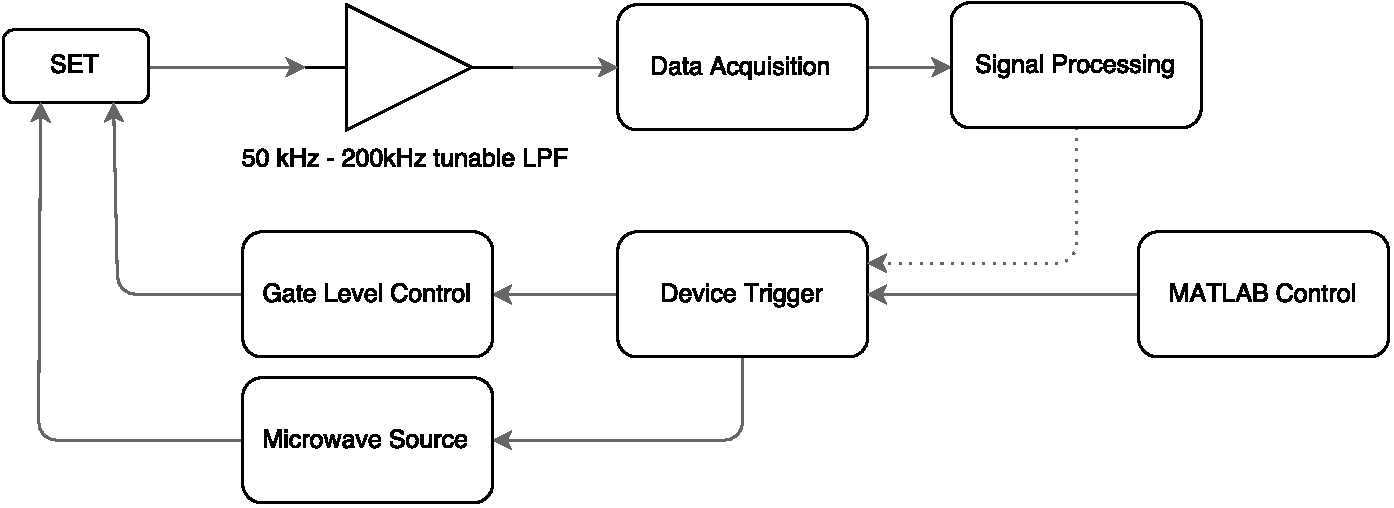
\includegraphics[width=\textwidth]{thesis_experiment.pdf}
	\caption{Block diagram of experiment}
	\label{fig::thesis_experiment}
\end{figure}

\begin{figure}[htbp!]
	\centering
	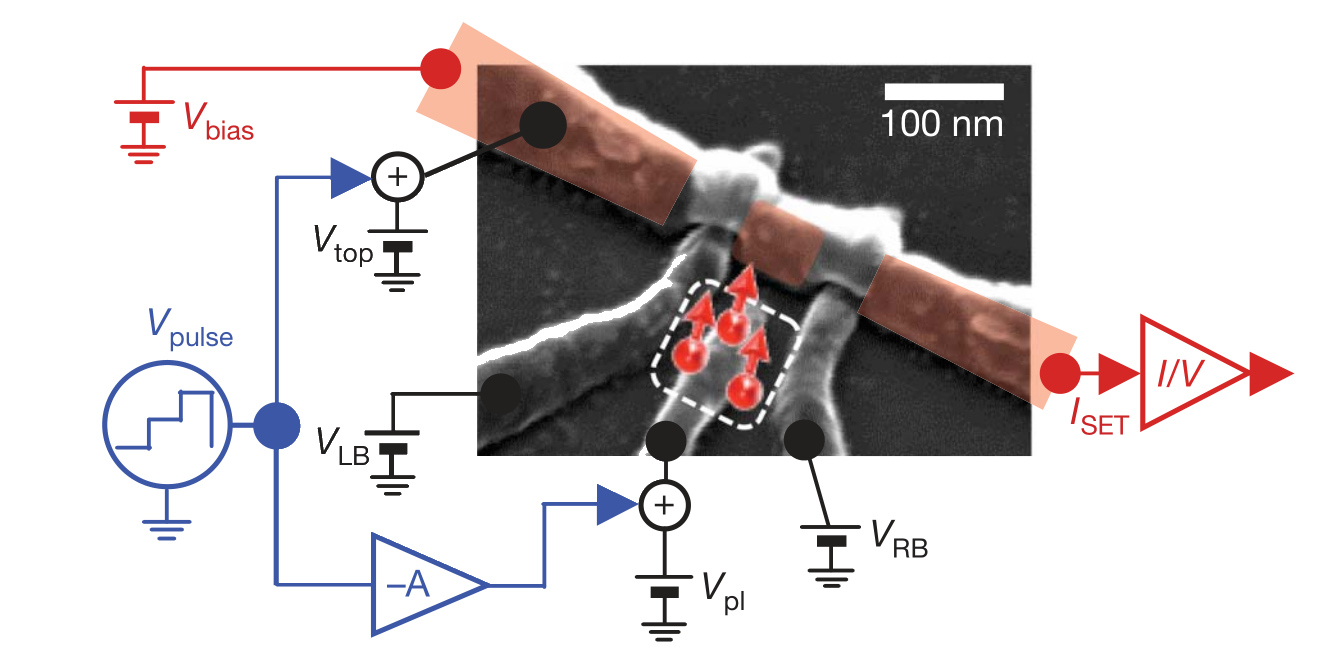
\includegraphics[width=\textwidth]{set_layout}
	\caption{The layout of an SET}
	\label{fig::set_layout}
\end{figure}

\begin{figure}[htbp!]
	\centering
	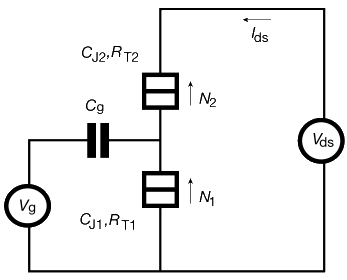
\includegraphics[width=0.6\textwidth]{set_circuit}
	\caption{Equivalent electrical circuit of an SET}
	\label{fig::set_circuit}
\end{figure}

\begin{figure}[htbp!]
	\centering
	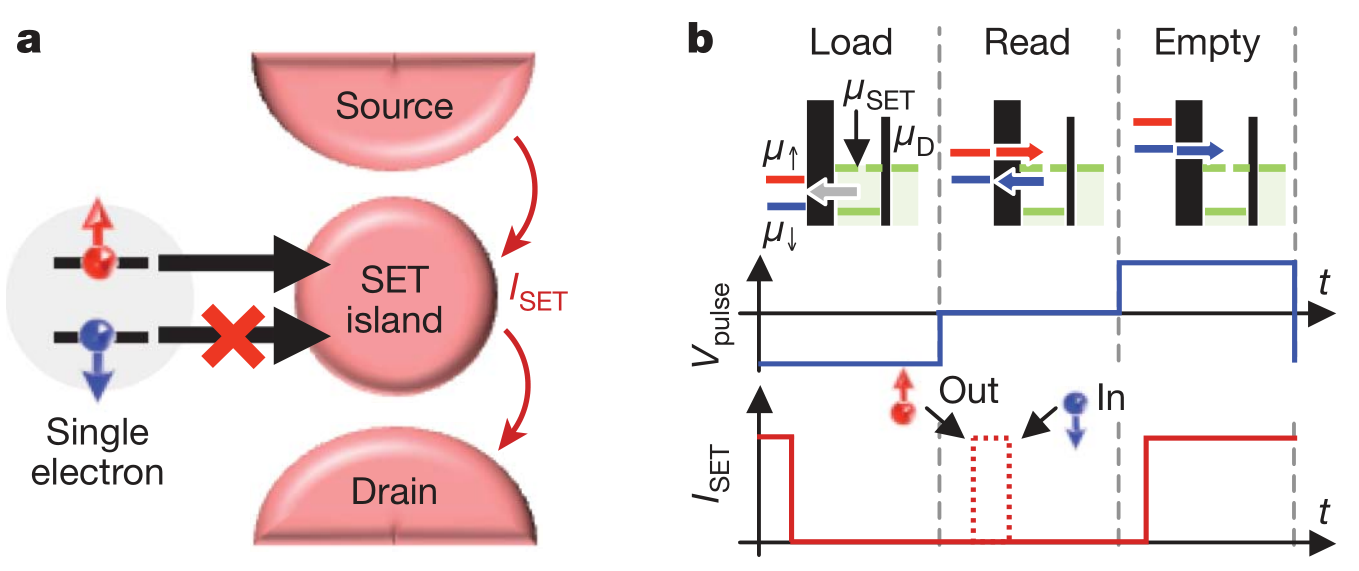
\includegraphics[width=\textwidth]{set_loading}
	\caption{The initialisation procedure of an SET}
	\label{fig::set_loading}
\end{figure}